Dataflow models expose concurrency. While concurrency enables parallelism, it can also be leveraged in other ways. 
This section discusses \"{Y}auhau, a framework for optimizing \ac{I/O} in microservice-based systems~\cite{ertel_cc18}.\index{\"{Y}auhau}
This Ohua-based framework uses the concurrency exposed by the \ac{MoC} to do so.

\begin{figure}[t]
        \centering
        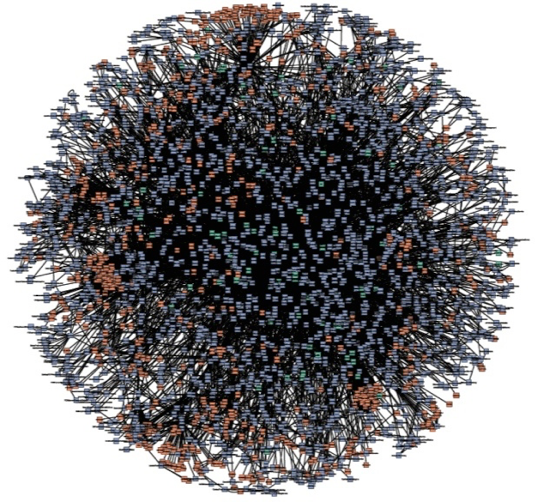
\includegraphics[scale=0.25]{figures/amazon-microservices.png}\\
        \small

        [Source: \href{https://www.slideshare.net/apigee/i-love-apis-2015-microservices-at-amazon-54487258}{I Love APIs 2015} by Chris Munns, licensed under \href{https://creativecommons.org/licenses/by/4.0/}{CC BY 4.0}, available at: \href{http://bit.ly/2zboHTK}{\url{http://bit.ly/2zboHTK}}]
        \vspace{-1mm}
        \caption{Microservices at Amazon.}
        \label{fig:amazon_death_star}
        \vspace{-3mm}
\end{figure}

The infrastructure of large internet companies today relies to a great extent on microservice-based architectures~\cite{decandia2007dynamo,marlow2014haxl}.
Figure~\ref{fig:amazon_death_star} shows the microservice infrastructure of Amazon circa 2015. 
It shows microservices as nodes, and how they depend on each other as edges.
The figure serves to illustrate the complexity of microservice-based architectures.

In microservice-based systems, \ac{I/O} plays a crucial role in the performance.
A microservice will commonly send multiple requests to a different microservice, as part of its operation.
Each request comes with a significant overhead from establishing the connection and sending the data.
If the requests do not depend on each other, however, they can instead be sent as a single, batched request for mitigating the overhead.

Batching requests is not a novel idea, it is well-established as a technique to optimize \ac{I/O}.
The trade-off comes from the code required to write batched requests.
A developer writing code for such a microservice-based architecture needs to take both the funcionality and the \ac{I/O} optimizations into account.
This makes the code harder to write, read and mantain, as the optimizations clutter the readability of the functionality.
This is unacceptable in a context where development time is a highly valuable resource, be it for human-resource costs or because it is important to have working solution as quick as possible. 

The suituation described is the case for Facebook's spam-fighting services~\cite{marlow2014haxl}.
When fighting spam, a novel filter must not only be effective and perform efficiently, it also should be implemented as fast as possible without compromising the functionality.
An ideal spam-fighting system thus allows the developers to focus on the functionality, and optimizes the implementation without cluttering the code.
This is precisely what the Haxl\index{Haxl} sytem attempts, using the Haskell abstraction of \emph{applicative functors}\index{applicative functor}.
Consider the Haskell code snippet (taken from \cite{marlow2014haxl}) in Listing~\ref{listing:haxl_friends_of}:

\begin{listing}[h]
\begin{minted}[]{Haskell}
let numCommonFriends =
     length (intersect (friendsOf x) (friendsOf y))
in
if numCommonFriends < 2 && daysRegistered x < 30
    then...
    else...
\end{minted}
\caption{An example of a Spam-fighting request to be optimized by Haxl (from ~\cite{marlow2014haxl}).}
\label{listing:haxl_friends_of}
\end{listing}

The listing shows a code example where, for spam fighting, the number of common Facebook friends of two users are calculated.
This is done by calling the function \texttt{friendsOf} for both \texttt{x} and \texttt{y}.
Code like Listing~\ref{listing:haxl_friends_of} is easy to read, but unoptimized, it will send to requests to the microservice that handles the \texttt{friendsOf} function.
The solution of Haxl is to use applicative functors to compose \ac{I/O} calls, such as \texttt{friendsOf}, and automatically batch independent requests this way.
Listing~\ref{listing:haxl_appliactive_do} shows how this is achieved in Haxl using applicative-do notation.

\begin{listing}
\begin{minted}[]{Haskell}
do a <- friendsOf x
   b <- friendsOf y
   return (length (intersect a b))
\end{minted}
\caption{The request from Listing~\ref{listing:haxl_friends_of} batched using applicative-do (from ~\cite{marlow2014haxl}).}
\label{listing:haxl_applicative_do}
\end{listing}

Under the hood, the applicative functor definition for \texttt{friendsOf} in Haxl gathers the arguments \texttt{x} and \texttt{y} and makes a single, batched request.
This optimizes the execution with a minimal obfuscation of the code:
A developer has to switch from a pure functional style to an applicative style, but can otherwise focus on the semantics of the program.

Our central observation is that this \ac{I/O} optimizations all come ``for free'' from the exposed concurrency in a dataflow execution. 
If we define a dataflow operator that gathers the inputs and issues a single batched request, we get the composition from the semantics of dataflow.
This is the main idea behind \"{Y}auhau.


\"{Y}auhau is based on the iteration of Ohua embedded in Clojure.
It is a language with an explicit annotation for functions which perform \ac{I/O}.
Leveraging these annotations, a semantics-preservig transformation can minimize the number of independent \ac{I/O}-performing function calls.
We map the Clojure-based Ohua to an internal expression \acsu{IR}, as is shown in Figure~\ref{fig:clojure_to_yauhau}.

\begin{figure}[h]
	\centering
	\begin{tabular}{r r c l r r r c l r}
		&\mintinline{Clojure}{x} & $\mapsto$ & $x$ &  &\mintinline{Clojure}{(let [x t] t)} & $\mapsto$ & $\lit*{let} \: x = t \: \lit*{in} \: t$ &  \\

	&\mintinline{Clojure}{(io x)}&$\mapsto$& $\lit*{io}(x)$ & &\mintinline{Clojure}{(fun [x] t)} $\equiv$ \mintinline{Clojure}{#(t)} & $\mapsto$ & $\lambda x.t$ &\\ 
	&\mintinline{Clojure}{(t t)} & $\mapsto$ & $t \: t$ &	 &\mintinline{Clojure}{(f x1 ... xn)} & $\mapsto$ & $\lit*{ff}_f(x_1 \ldots x_n)$ & \\
    & & & & &	\mintinline{Clojure}{(if t t t)} & $\mapsto$ & $\lit*{if}(t \: t \: t)$  	%		\\
		%		\multicolumn{4}{l}{\textit{Values:}}\\
		%		&\mintinline{Clojure}{(reqF x1 ... xn)}& $\mapsto$ & $r_f$ & \\
	\end{tabular}
	
	\caption{Mapping the terms of the Clojure-based language to an expression \acs{IR}. Adapted from Figure~9 in~\cite{ertel_cc18}.}
	\label{fig:clojure_to_yauau}
\end{figure}

The expression \ac{IR} defined in Figure~\ref{fig:clojure_to_yauau} is based on $\lambda$ calculus with a \texttt{let} construction for lexical scoping and explicit conditionals (\texttt{if}).
The central innovations of the language are the two particular terms, \texttt{ff} for foreign functions, which is any (possibly stateful) function.
The other term is \texttt{io}, which is an explicit annotation that a function does \ac{I/O}\index{\"{Y}auhau ! io}.
The premise is to optimize the number of annotated \ac{I/O} calls leveraging the concurrency from the dataflow semantics derived from this language.
The example in Listing~\ref{listing:yauhau_friends_of} lists the same request as Listing~\ref{listing:haxl_friends_of} in \"{Y}auhau.

\begin{listing}
\begin{flalign*}
& \lit*{let}~\lit*{numCommonFriends} = & \\ 
& \quad \lit*{ff}_\text{length}(\lit*{ff}_\text{intersect}( & \\ 
& \quad \quad \lit*{ff}_\text{friendsOf}(\lit*{io}(x)),~\lit*{ff}_\text{friendsOf}(\lit*{io}(y)) & \\
& \quad ))~\lit*{in}~\ldots & 
\end{flalign*}
\caption{The request from Listing~\ref{listing:haxl_friends_of} in \"{Y}auhau.}
\label{listing:yauhau_friends_of}
\end{listing}

The \ac{I/O} optimizations in \"{Y}auhau come from batching requests.
Instead of calling \texttt{ff}$_\text{friendsOf}$(\texttt{io}(\texttt{x})) and \texttt{ff}$_\text{friendsOf}$(\texttt{io}(\texttt{y})) as two separate \ac{I/O} requests, we can call them as a single batched request, since they are independent.
In \"{Y}auhau we do so by introducing a \emph{batched} \ac{I/O} statement, \texttt{bio}\index{batched \acs{I/O}}.
The \texttt{bio} statement takes a list of arguments and does a batched call with this list.
In the example, the two statements become a single \texttt{ff}$_\text{friendsOf}$(\texttt{bio}(\texttt{[x,y]}).

Through semantics-preserving transformations using \texttt{let} floating we can get independent \ac{I/O} calls batched this way and transform them to dataflow.
The explicit concurrency in the dataflow transformation allows to execute batched \ac{I/O} calls when they arrive.
The details of the transformation~\cite{ertel_cc18} are beyond the scope of this thesis.
We discuss how we evaluate the effectiveness of the transformation using the Level Graphs methodology described in Section~\ref{sec:level_graphs}.


\begin{figure}[t]
    	\centering
      \resizebox{0.95\textwidth}{!}{
        \inputTikz{yauhau_baseline}
      }
		\caption{Batching \ac{I/O} with \"{Y}auhau compared to Haxl and Muse. Adapted from Figure~11 of~\cite{ertel_cc18}.}	
		\label{fig:yauhau_baseline}
\end{figure}

Figure~\ref{fig:yauhau_baseline} shows a comparison of our framework, \"{Y}auhau, with the two other main alternatives in the public domain, Facebook's Haxl~\cite{marlow2014haxl} and Muse~\cite{muse}.
We cannot compare with Twitter's Scala-based variant, Stitch\cite{stitch}, which is neither described in a peer-reviewed publication nor open-sourced.
Since we do not have a real test workload like Facebook does to reproduce the evaluation of~\cite{marlow2014haxl}, we used synthetic graphs with a similar structure to compare the approach.s
We produced random Level Graphs with code annotations as described in Section~\ref{sec:level_graphs}. 
We varied the number of levels between $1$ and $20$ in the generated graph.
An increasing number of levels results in increasingly complex applications and interactions.
For this baseline comparison we disabled sub-functions by letting the probability of labeling a node as a sub-function be $0$.
For each number of levels we generated $20$ graphs and produced code for each of the frameworks with the structure of each of these twenty graphs.
This way the same workload is evaluated for each framework, as equivalent versions are produced from a single graph.
The number of \ac{I/O} accesses in each individual graph is random nevertheless, which is why we used $20$ graphs per considered number of levels to obtain a statistical assessment of the batching effect of each framework.

The results of Figure~\ref{fig:yauhau_baseline} show that both Haxl and Muse consistently batch \ac{I/O} calls, improving over a sequential execution in a statistically significant fashion.
The ratio of \ac{I/O} calls compared to a sequential execution improves with increasing code complexity, as measured by the number of levels. 
Compared to Haxl and Muse, which produce equivalent results, \"{Y}auhau batches significantly more \ac{I/O} calls.
The reason for \"{Y}auhau beating the other two frameworks is that it can batch across multiple levels, due to the underlying dataflow representation.
Both Haxl and Muse work in \emph{rounds}, which depend on the code structure.
Thus, to fully optimize \ac{I/O} in these frameworks, developers need to re-organize their code to maximize batch requests in each round.
This partially defeats the purpose of the \ac{DSL}, namely to free developers from performance concerns and let them focus solely on the functionality.

\begin{figure}[t]
    	\centering
      \resizebox{0.95\textwidth}{!}{
        \inputTikz{yauhau_concurrency}
      }
		\caption{Concurrent \ac{I/O} with \"{Y}auhau compared to Haxl and Muse. Adapted from Figure~12 of~\cite{ertel_cc18}.}	
		\label{fig:yauhau_io-imbalance}
	\end{figure}

Figure~\ref{fig:yauhau_io-imbalance} shows a second experiment, where concurrency in \ac{I/O} is enabled in the dataflow graph.
Since Haxl and Muse are equivalent in terms of their batching, we just compare to Haxl in this experiment.
We compare \"{Y}auhau to a variant which blocks computation when performing \ac{I/O} and a concurrent dataflow variant.
Again we use level graphs to produce benchmarks tailored to our problem, this time we add a fixed (randomly-chosen) execution time for the computation and \ac{I/O} nodes in the graph, to simulate the computation time and \ac{I/O} latency.
We see how the concurrency of the dataflow \ac{MoC} improves the latency of the service significantly beyond the additional benefits already provided by the round-free batching.

Finally, an important advantage of the dataflow \ac{MoC} we have not evaluated is how it also allows us to transcend the function boundaries.
To test this we can again leverage the full control we get from our Level Graph benchmarking method.
We fix the number of levels, controlling the code complexity, and consequently the average number of \ac{I/O} requests.
Instead of varying the number of levels, we allow sub-function and vary the probability of generating such a sub-function.
The higher the probability, the more nested functions appear in the code.
In other words, we can make code with similar levels of complexity be more or less modular.
This allows us to test directly how modularity affects batching.

\begin{figure}[t]
	\centering
      \resizebox{0.95\textwidth}{!}{
        \inputTikz{yauhau_functions}
      }
	\caption{Concurrent \ac{I/O} in modular programs with \"{Y}auhau. Adapted from Figure~13 of~\cite{ertel_cc18}.}
	\label{fig:yauhau_efficient-modularity}
\end{figure}

Figure~\ref{fig:yauhau_efficient-modularity} shows the results of the modularity experiment.
For this case, Haxl and Muse differ, since our Haxl back-end uses applicative-do desugaring, which allows the compiler to optimize more than in Muse.
Most notably however, both Haxl and Muse significantly increase the amount of \ac{I/O} requests when the program becomes more nested, while in \"{Y}auhau this is not the case.
This is because of the underlying dataflow \ac{MoC}, which flattens the dependency graph, effectively inlining the sub-function calls and allowing the framework to batch across function boundaries.
In particular, this means again that the premise of making developers not worry about performance in the \ac{DSL} is partially broken by Haxl and Muse, and this is fixed by \"{Y}auhau.

We have seen how \ac{MoC}-based design can be useful in context different from the \ac{CPS} applications we focused on in the previous chapters.
In particular, the Ohua approach can be used to make the model more implicit in the computation, which is crucial for developer adoption in many contexts.
Finally, we have seen in this section as well some of the concrete advantages of random benchmarks with a clearly-defined structure, in the concrete example of the Level Graphs from Section~\ref{sec:level_graphs}.
They allowed us to tailor experiments to isolate specific features of our dataflow \ac{MoC}-based approach and compare them to the other state-of-the-art approaches.